174. \begin{figure}[ht!]
\center{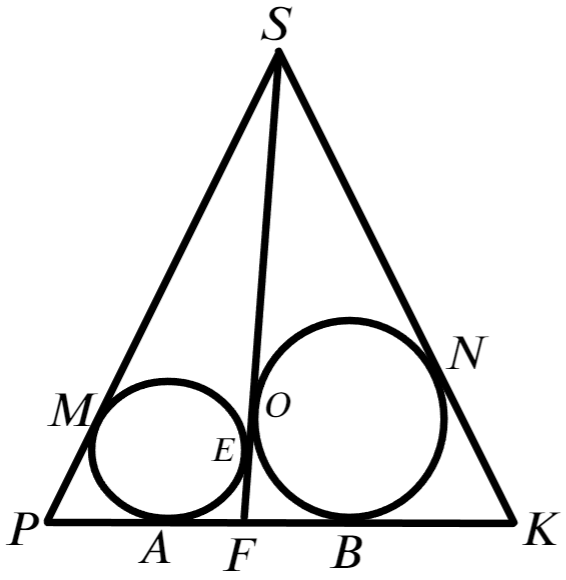
\includegraphics[scale=0.35]{g9-174.png}}
\end{figure}\\
Так как $FK>PF,$ точка $O$ находится между $S$ и $E.$ Отрезки касательных, проведённых из одной точки, равны, отсюда имеем равенства $SE = SM,\ SO = SN,\ PM =
PA,\ KB = KN,\  FA = FE,\  FO = FB.$ Тогда $OE = SE - SO = SM - SN = (SP - PM) - (SK - NK) = NK - PM =
BK - AP = (FK - FB) - (FP - FA) = FA - FB + 2 = FE - FO + 2 =
2 - OE \Rightarrow 2OE = 2\Rightarrow OE=1.$\\
